% !TeX root = ../main.tex
% Add the above to each chapter to make compiling the PDF easier in some editors.

\chapter{Related Works}\label{chapter:related_works}


\section{Traditional Approaches for Prognostic and Health Management}

Generally, there exist model-based or data-driven PHM algorithms. Model-based methods predict the health condition based on physical models, which describe the underlying mechanisms of degradation. Uncertainties in the machine processes as well as noise make the application of physical models difficult. Besides that, identifying all model parameters might be difficult and requires a lot of experiments. Data-driven methods learn a mapping relationship between the health condition state and monitoring data. Such methods do not use physical information about the degradation process. The performance of data-driven approaches highly depends on the quality and amount of training data. Besides that data-driven models might lack from generality. The models are just optimized to perform well on those working conditions which are present in the train data. Both, model-based and data-driven approaches suffer from different limitations. The challenge of hybrid models lies in the integration framework, which bridges the processes of the data-driven and model-based approaches \cite{DENG2020}. In the following data-driven and model-based approaches are presented. 

\subsection{Model-Based Approach: Prognostics and Health Management with Defect Frequencies}
Lee et al \cite{Lee2015} propose a diagnosis system, which in first place determines characteristic frequencies for different machine defects. By searching for those defect frequencies in the machine signals, one can make predictions about current defect types and severity. Fig. \ref{fig:defect_frequency_model} visualizes the proposed approach.

\begin{figure}[H]
  \centering
  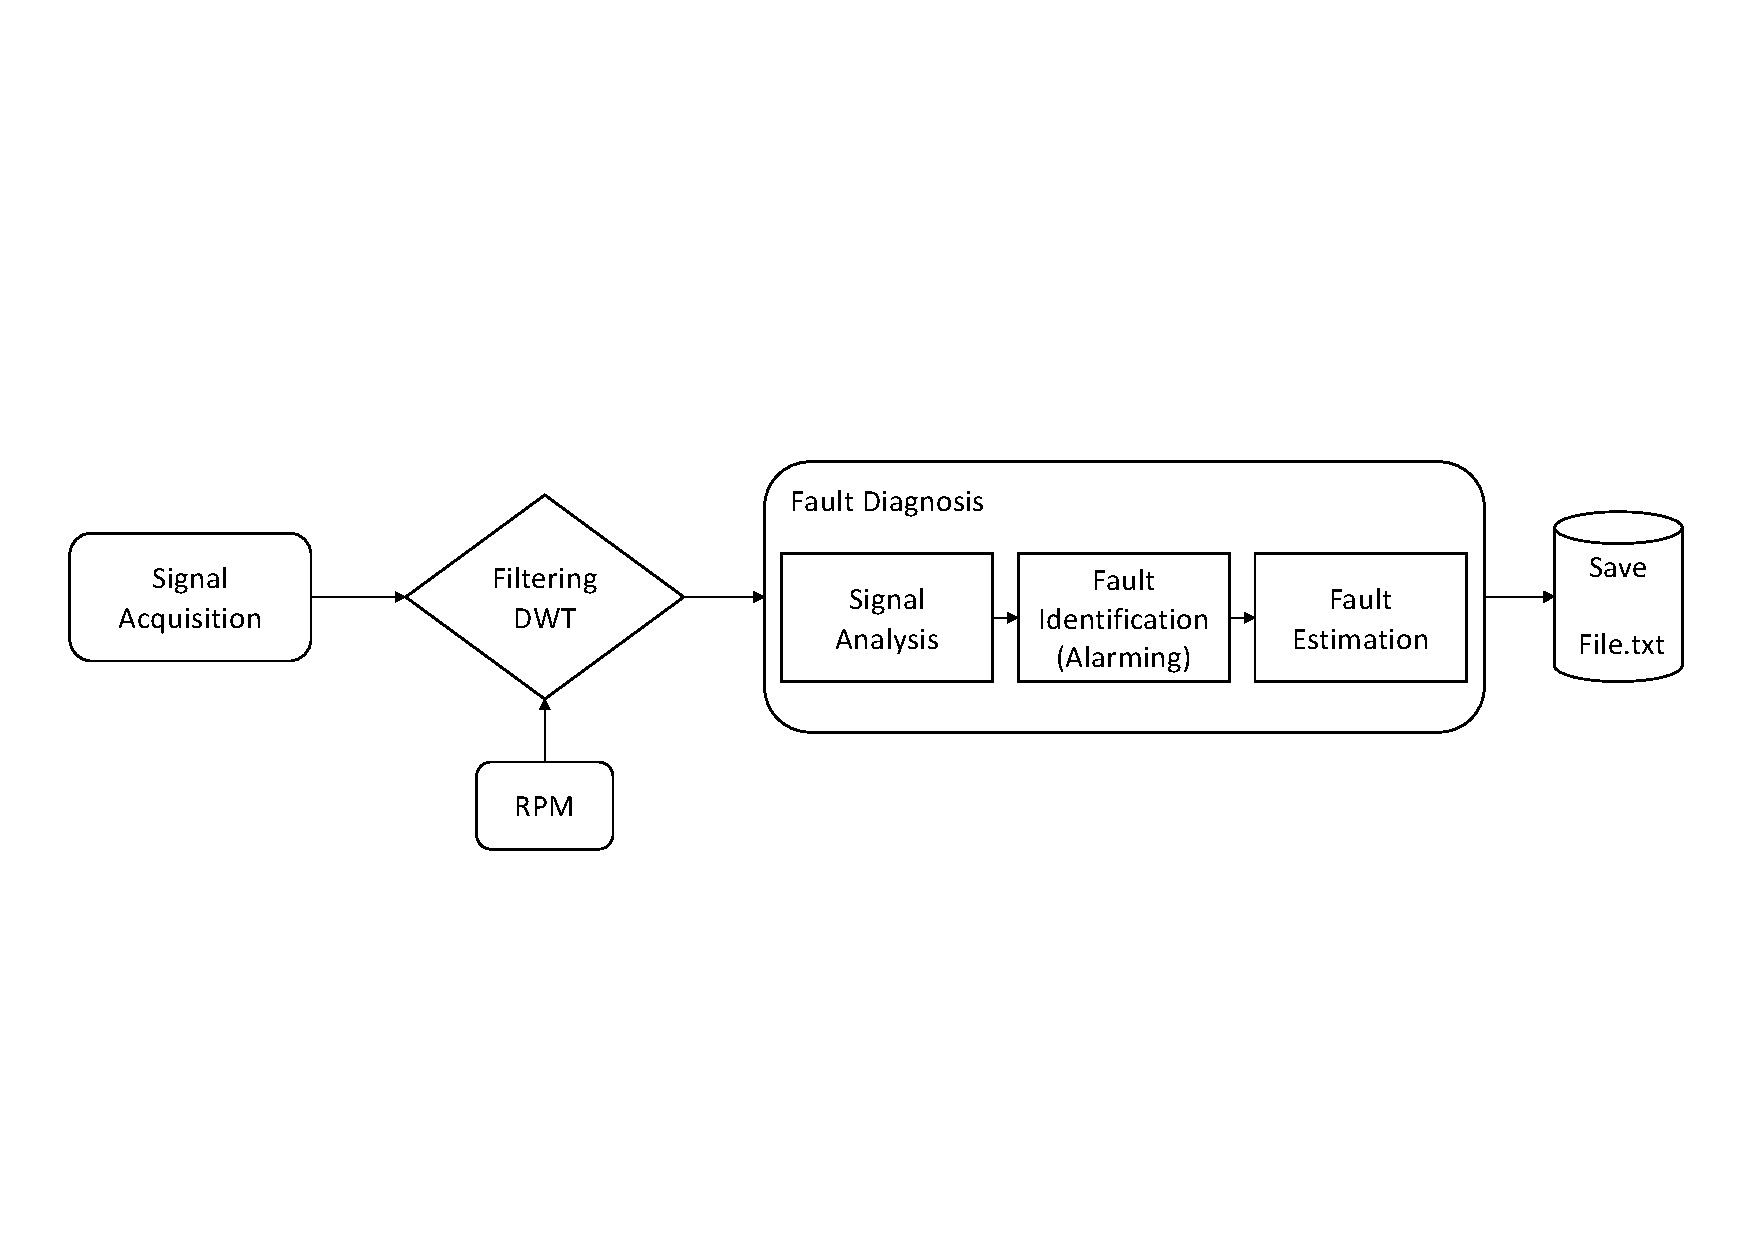
\includegraphics[width=.95\textwidth]{models_state_of_the_art/defect_frequency_model.pdf}
  \caption{Failure diagnosis system by calculating defect frequencies based on \cite{Lee2015}}
  \label{fig:defect_frequency_model}
\end{figure}

Lee et al use a method proposed by Harris and McCool \cite{Harris1996} to estimate the characteristic defect frequencies. This method treats the ball screw drives as a bearing, where the screw shaft is considered as inner and the nut as outer ring. From the construction details and the relative speed between the ball screw drive components, the defect frequencies can be calculated. 
Defect frequencies are described by the ball pass frequencies of shaft (BPFS), ball pass frequency of nut (BPFN), and ball spin frequency (BSF): 
\begin{equation}
    BPFS = \frac{1}{120}zn(1+\frac{D_{w}}{d_{m}}cos\alpha),
    \label{eq:defect_frequency}
\end{equation}
\begin{equation}
    BPFN = \frac{1}{120}zn(1-\frac{D_{w}}{d_{m}}cos\alpha),
\end{equation}
\begin{equation}
    BSF = \frac{1}{120}n\frac{d_{m}}{D_{w}} (1-\frac{D_{w}}{d_{m}}cos\alpha)(1+\frac{D_{w}}{d_{m}}cos\alpha) ,
\end{equation}
where $\alpha$ is the contact angle made by the ball, nuts, and screw shaft, $d_{m}$ is the pitch diameter of balls, $D_{w}$ is the diameter of each ball, the rotational speeds of external and internal races are $n_{e}$ and $n_{i}$, $z$ is the number of steel balls. The bearing parameters are visualized in fig. \ref{fig:defect_frequency_calc}. 

\begin{figure}[H]
  \centering
  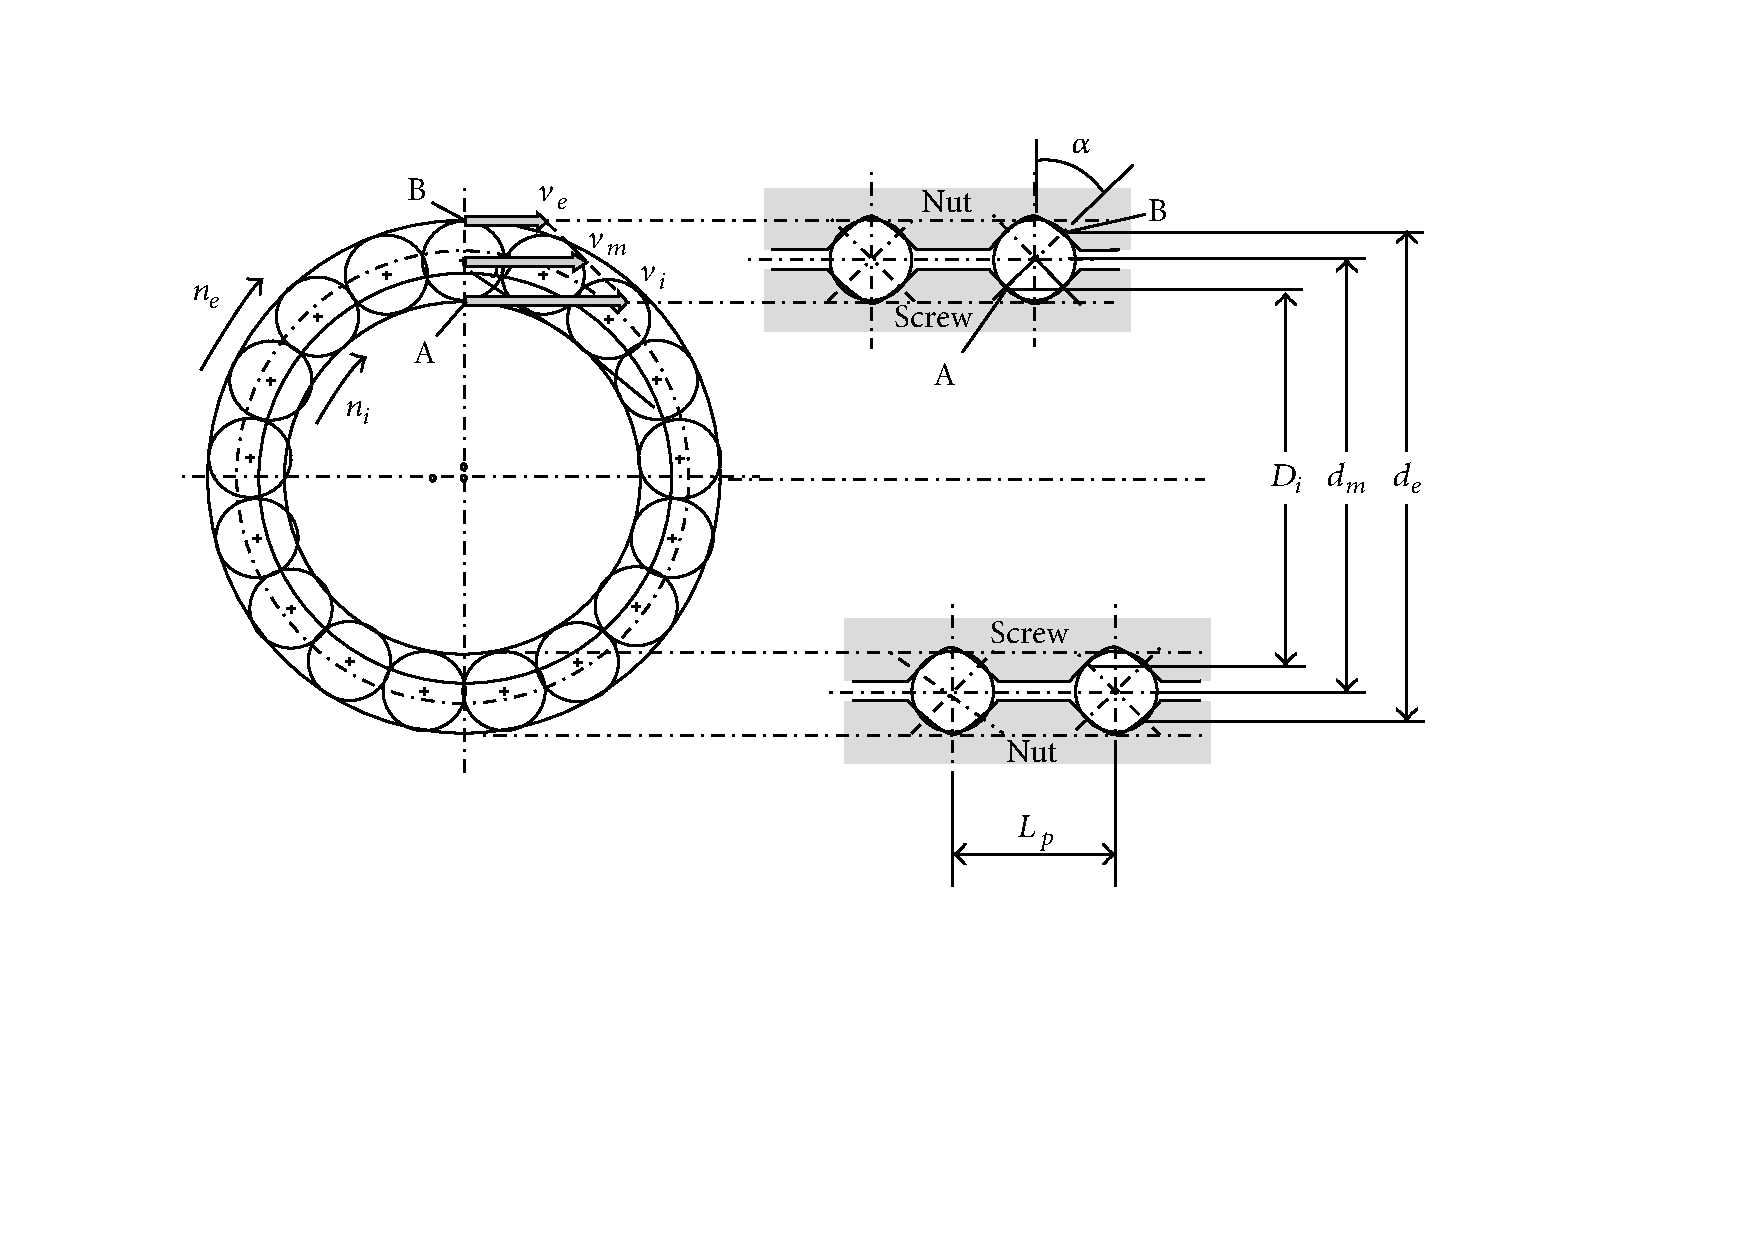
\includegraphics[width=.6\textwidth]{models_state_of_the_art/defect_frequency_calc.pdf}
  \caption{Simplification of BSDs as bearings for frequency calculation \cite{Lee2015}}
  \label{fig:defect_frequency_calc}
\end{figure}

The above derived frequencies are valid for bearings. To apply those to ball screw drives one has to replace $z$ and $d_{m}$ by the effective number of steel balls $z^{'}$ and effective pitch parameter $d_{m}^{'}$:

\begin{equation}
    d_{m}^{'} = (L_{p}^{2}+(\pi D_{b})^{2})^{\frac{1}{2}},
\end{equation}
\begin{equation}
    z^{'} = \frac{d_{m}^{'}}{D_{w}},
\end{equation}
where the meaning behind the used parameters is visualized in fig. \ref{fig:defect_frequency_transfer}. 

\begin{figure}[H]
  \centering
  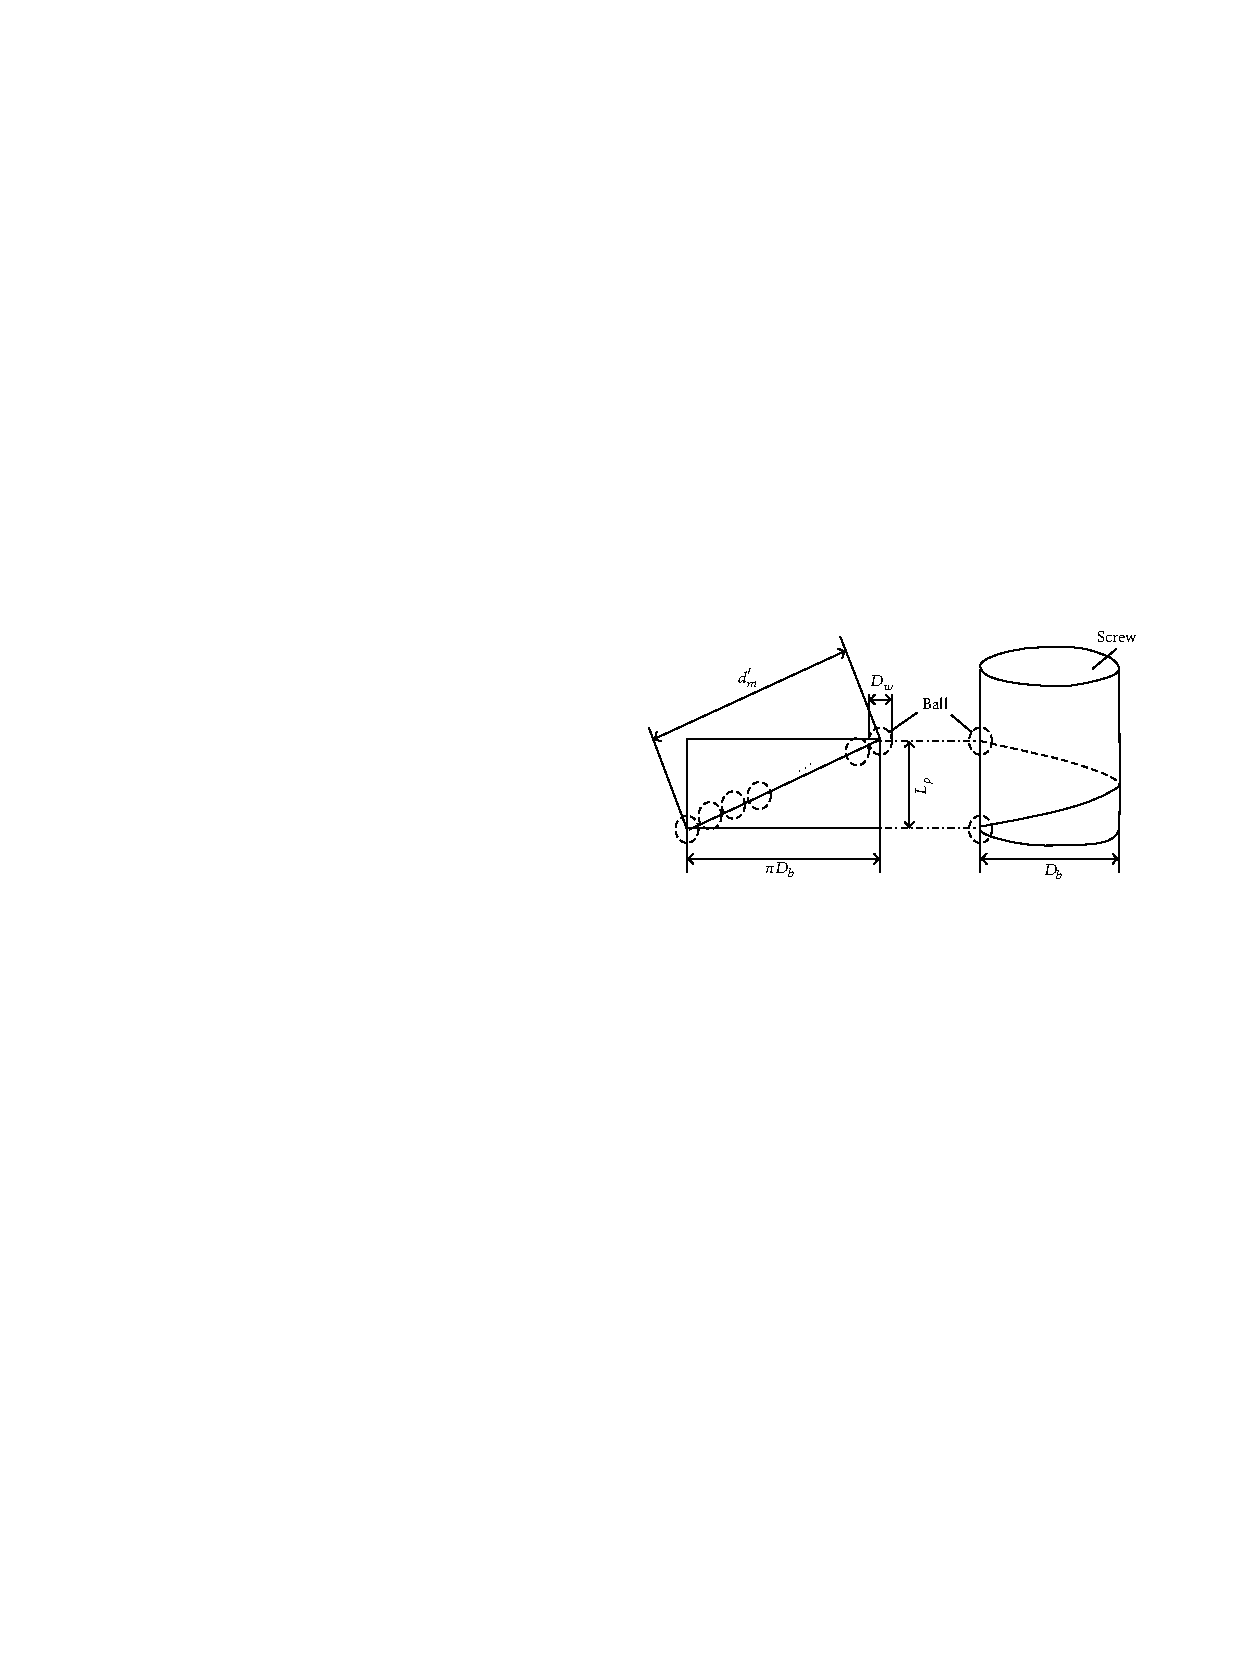
\includegraphics[width=.7\textwidth]{models_state_of_the_art/defect_frequency_transfer.pdf}
  \caption{Transfering pitch parameter and number of steel balls from bearings to BSDs \cite{Lee2015}}
  \label{fig:defect_frequency_transfer}
\end{figure}


The BPFS is the most expressive and reliable one for supervising the health condition of ball screw drives. To calculate the BPFS for ball screw drives the equation \ref{eq:defect_frequency} must be combined with $d_{m}^{'}$ and $z^{'}$. When monitoring the health condition of ball screw drives, the wavelet transform, specifically the Daubechies Wavelet (db14) function, is used to extract the frequencies from the signal. These frequencies can then be compared with the calculated defect frequencies. The amplitude of the detected characteristic defect frequency in the signal gives information about the degradation level of the ball screw drive.

\subsection{Data-Driven Approach: Sensor Fusion with Principal Component Analysis for Prognostics and Health Monitoring }

Denkena et al \cite{Denkena2021} present a method to monitor the loss of preload in ball screw drives. Several hand-crafted statistical features were extracted from the signals. A sensor fusion approach based on principle component analysis is used to combine those features. In the end decision trees are used to solve the classification task. Denkena et al separate the monitoring method in four steps:

\begin{itemize}
    \item [\textbf{Data acquisition:}] The method processes external control signals coming from three uniaxial acceleration sensors as well as internal control signals provided by the numerical control (NC) signals. The signals are concatenated and analyzed simultaneously.
    \item [\textbf{Data pre-processing:}] The signals are separated in parts of constant and changing ball screw drive speeds. 
    \item [\textbf{Feature extraction:}] Information about the preload classes are extracted through statistical features. The features are extracted for each signal and segment. Each feature is evaluated by its robustness and statistical significance. The robustness is measured by the feature's dispersion around the median. After normalizing the feature with the z-score, the significance is investigated by the f-statistics.
    
    \begin{equation}
        \textbf{Z-score:}\qquad \tilde{x}_{i,j} = \frac{x_{i,j} - \bar x_{i}}{\sigma_{i}},
    \end{equation}
    
    \begin{equation}
        \textbf{F-statistic:}\qquad f = \frac{\sum_{j=1}^{J} i \cdot (\bar x_{j} -\bar x)^{2}/(J-1)}{\sum_{j=1}^{J} \sum_{i=1}^{I} i \cdot (\bar x_{j,i} -\bar x_{j})^{2}/(J \cdot (I-1))},
    \end{equation}

    where ${x}_{i,j}$  denotes the feature value j for class i, $\bar {x}_{i}$ is the mean value,  ${s}_{i}$ is the standard deviation of the feature, I and J is the number of all features and classes. Denkena et al see features as eligible for the diagnosing system if the dispersion around the median is smaller than $\pm$ 10 and the f-statistics is higher than the critical value of 10. The selected features are merged with the goal of maintaining the robustness and increasing the f-statistics. The principal-component analysis is used to reduce the dimensions on the first two components.
    

    \item [\textbf{Classification:}] Denkena et al decided to use a decision trees to predict a preload class based on the extracted features. Due to its low classification effort and good traceability  decision trees seem suitable for the classification task. For each signal and segment a separate decision tree is used. 
\end{itemize}



\section{Domain Adaptation Approaches for Prognostic and Health Management of Ball Screw Drives}
In recent years, more and more intelligent and adaptive data-driven approaches were proposed for PHM in industrial machines. In the literature deep-learning based domain-adaption is a hot topic. With its origin in the computer vision community it slowly makes its way into the PHM domain. In the following, different deep-learning based domain adaption PHM systems for BSDs are presented. Similarly to the proposed method in this thesis they use a MMD loss to reduce the domain discrepancy.

\begin{comment}
\subsection{Deep Distance Metric Learning}
A PHM algorithm for rolling bearings, which optimizes the inter- and intra-class distance in the latent feature space and reduces the domain discrepancy with an MMD-loss, was presented by Li et al \cite{Li2018}. As visualized in fig. \ref{fig:Deep_distance_metric_learning_model} the model proposed by Li et al contains a CNN and a consecutive classifier. In a pre-processing step the raw vibration signal is first transformed in the frequency domain by applying wavelet transforms. Max-pooling layers are included to reduce the data dimension. Batch-normalization layers are used to reduce the internal-covariate-shift by normalizing the input distributions of the hidden layers. As a regularization method dropout layers with a rate of 0.5 help to avoid overfitting. 

\begin{figure}[H]
  \centering
  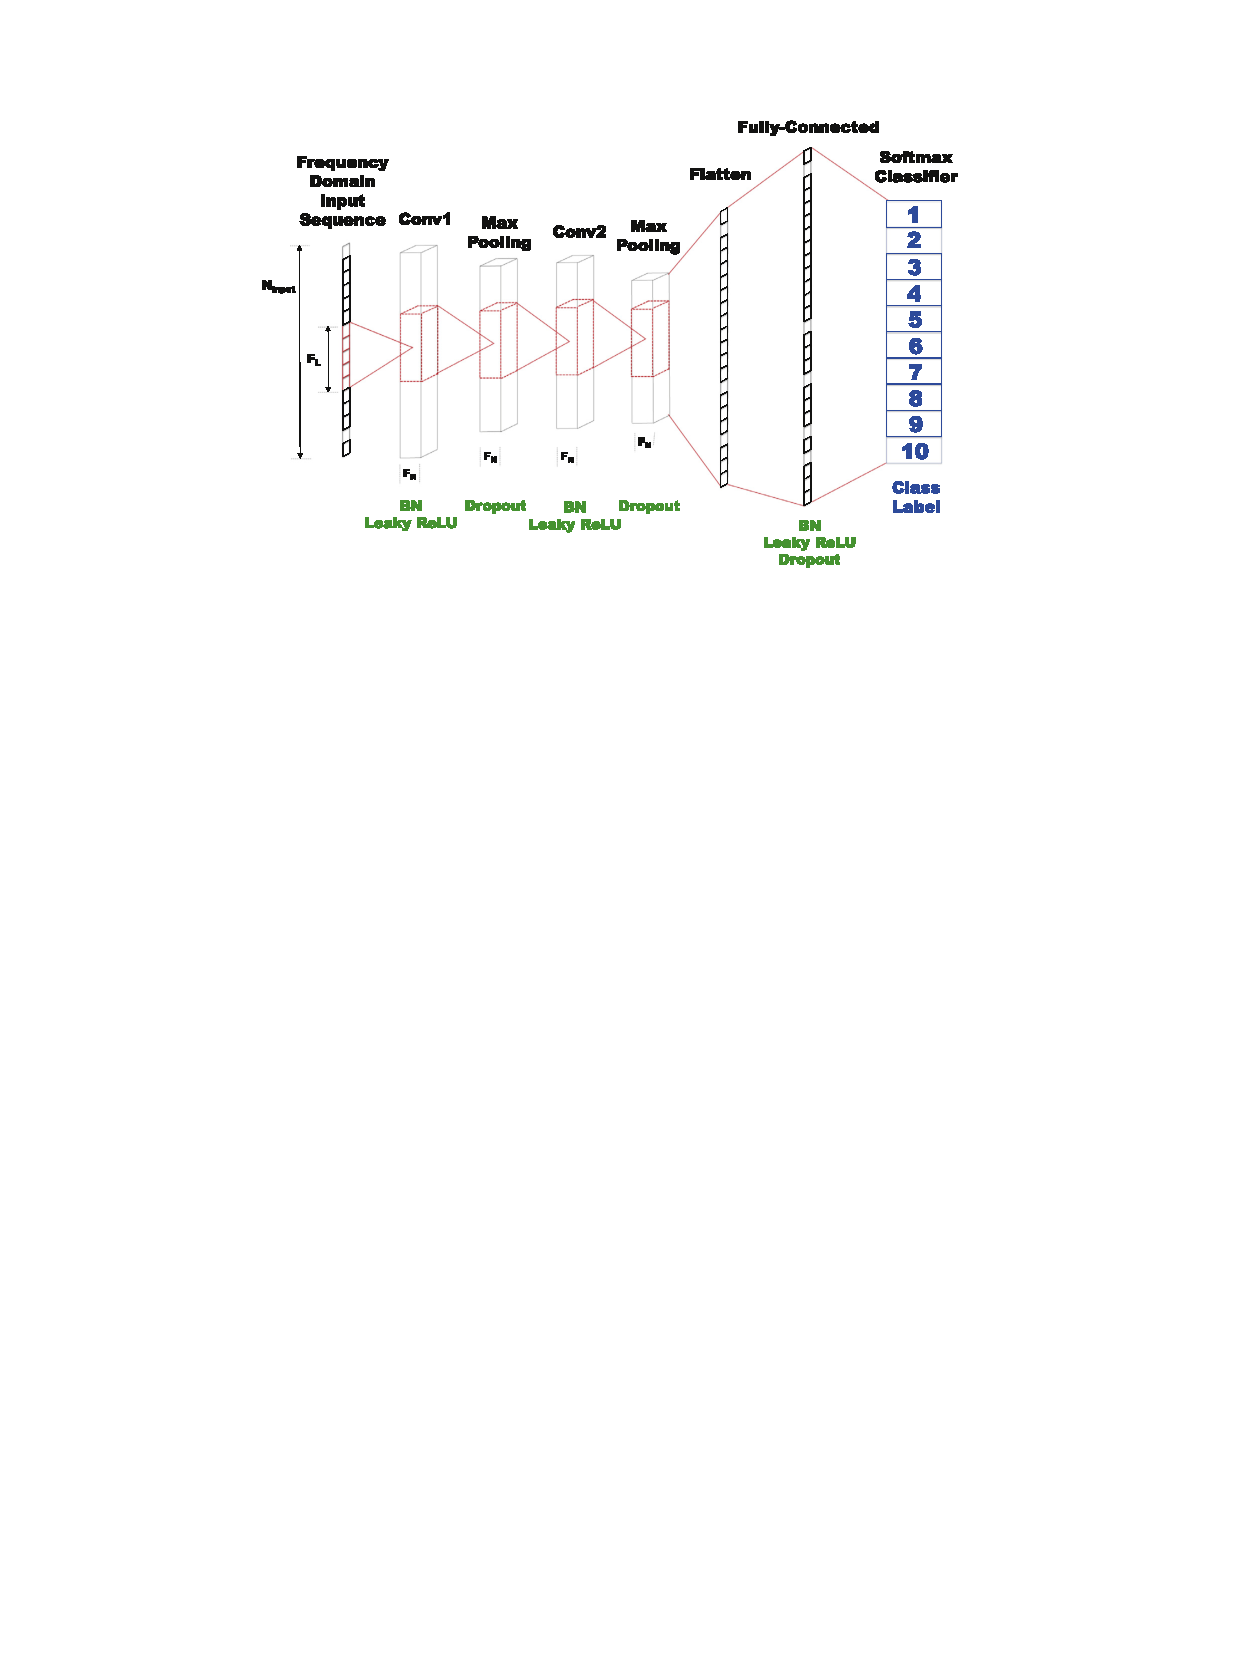
\includegraphics[width=.75\textwidth]{models_state_of_the_art/Deep_distance_metric_learning_model.pdf}
  \caption{Deep distance metric learning architecture proposed by Li et al \cite{Li2018}}
  \label{fig:Deep_distance_metric_learning_model}
\end{figure}

Li et al suggest to optimize the model such that the distance between samples of the same class is minimized and maximized between those of different classes. This increases the separability between as well as the compactness within the classes, which makes the algorithm more robust against environmental noises. In order to calculate the intra- and inter-class distances the expectation and variance of source domain samples belonging to the same class need so be measured in the feature maps of interest:

\begin{equation}
    \begin{aligned}
       &D_{inter} = |E[f^{(m)}x^{(i)}]-E[f^{(m)}x^{(j)}]|_{2}-\sqrt{Var[f^{(m)}x^{(i)}]}-\sqrt{Var[f^{(m)}x^{(j)}]}\\
       &D_{intra} = 
        \sum_{i=1}^{N_{class}} \sqrt{Var[x^{(i)}]},
    \end{aligned}
\end{equation}

where $x^{(k)}$ denotes the raw input sample of class k, $N_{class}$ is the number of classes, $f^{(m)}x^{(k)}$ denotes the feature representation of the input sample $x^{(k)}$ in the m-th layer and $E[f^{(m)}x^{(i)}]$ and $Var[f^{(m)}x^{(i)}]$ are the corresponding expectation and variance of this feature map. Optimizing the network with $\min_{f^{(m)}}J_{Cluster} = - D_{inter} + \eta D_{intra}$ maximizes the inter- and reduces the intra-class distance. Since $J_{Cluster}$  requires labels for each sample, the optimization is restricted to source domain data. Furthermore, Li et al applies a MMD-loss to reduce the discrepancy between target and source domain: 

\begin{equation}
    \begin{aligned}
    J_{MMD,m} = MMD_{k}(P^{f(m)}, Q^{f(m)}),
    \end{aligned}
\end{equation}

where $P^{f(m)}$ and $Q^{f(m)}$ denote the representation of source and target samples in the m-th hidden layer. Lastly, a CE-loss in the final layer optimizes the network to classify the source samples correctly. In total, the network is optimized with the following weighted average of losses: 

\begin{equation}
    \begin{aligned}
    J_{total} = \alpha J_{Cluster} + \beta J_{MMD} + \gamma J_{CE}, 
    \end{aligned}
\end{equation}
where $J_{Cluster}$ is the cluster loss, $J_{MMD}$ the MMD-loss,  $J_{CE}$ the CE-loss and $\alpha$, $\beta$ and $\gamma$ are the weights for calculating the weighted average \cite{Li2018}.


\subsection{Deep Convolutional Transfer Learning Network}
PHM of rolling bearing is a task with high demand in the industry. Guo et al \cite{Guo2019} propose a deep convolutional transfer learning network (DCTLN), which reduces the domain discrepancy by applying a MMD-loss and domain classifier. The architecture of the model is visualized in fig. \ref{fig:DCTLN_model}. Features are extracted by a CNN containing 16 layers including one input layer, six convolutional layers, six pooling layers, two fully connected layers, and one output layer. Each convolutional layer is combined with a consecutive pooling layer.


The model is optimized with a combination of three losses
\begin{itemize}
    \item [1.] Reduce the health condition classification loss on the source domain data
    \item [2.] Maximize the domain classification loss on the source and target domain 
    \item [3.] Minimize the MMD distance between the source and target domain in the FC2 layer
\end{itemize}

\textbf{Objective 1}: By applying the CE-loss the model training minimizes the health condition classification error on the source domain data.

\textbf{Objective 2}: The domain classifier processes the features in the layer FC3 and tries to predict the corresponding domain of each sample. The model is trained to extract domain invariant features such that the error of the domain classifier is increased.

\textbf{Objective 3}: The MMD-loss is applied in the feature map FC2. The model is optimized to decrease the domain discrepancy and to extract more domain invariant features in FC2 \cite{Guo2019}. 

\begin{figure}[H]
  \centering
  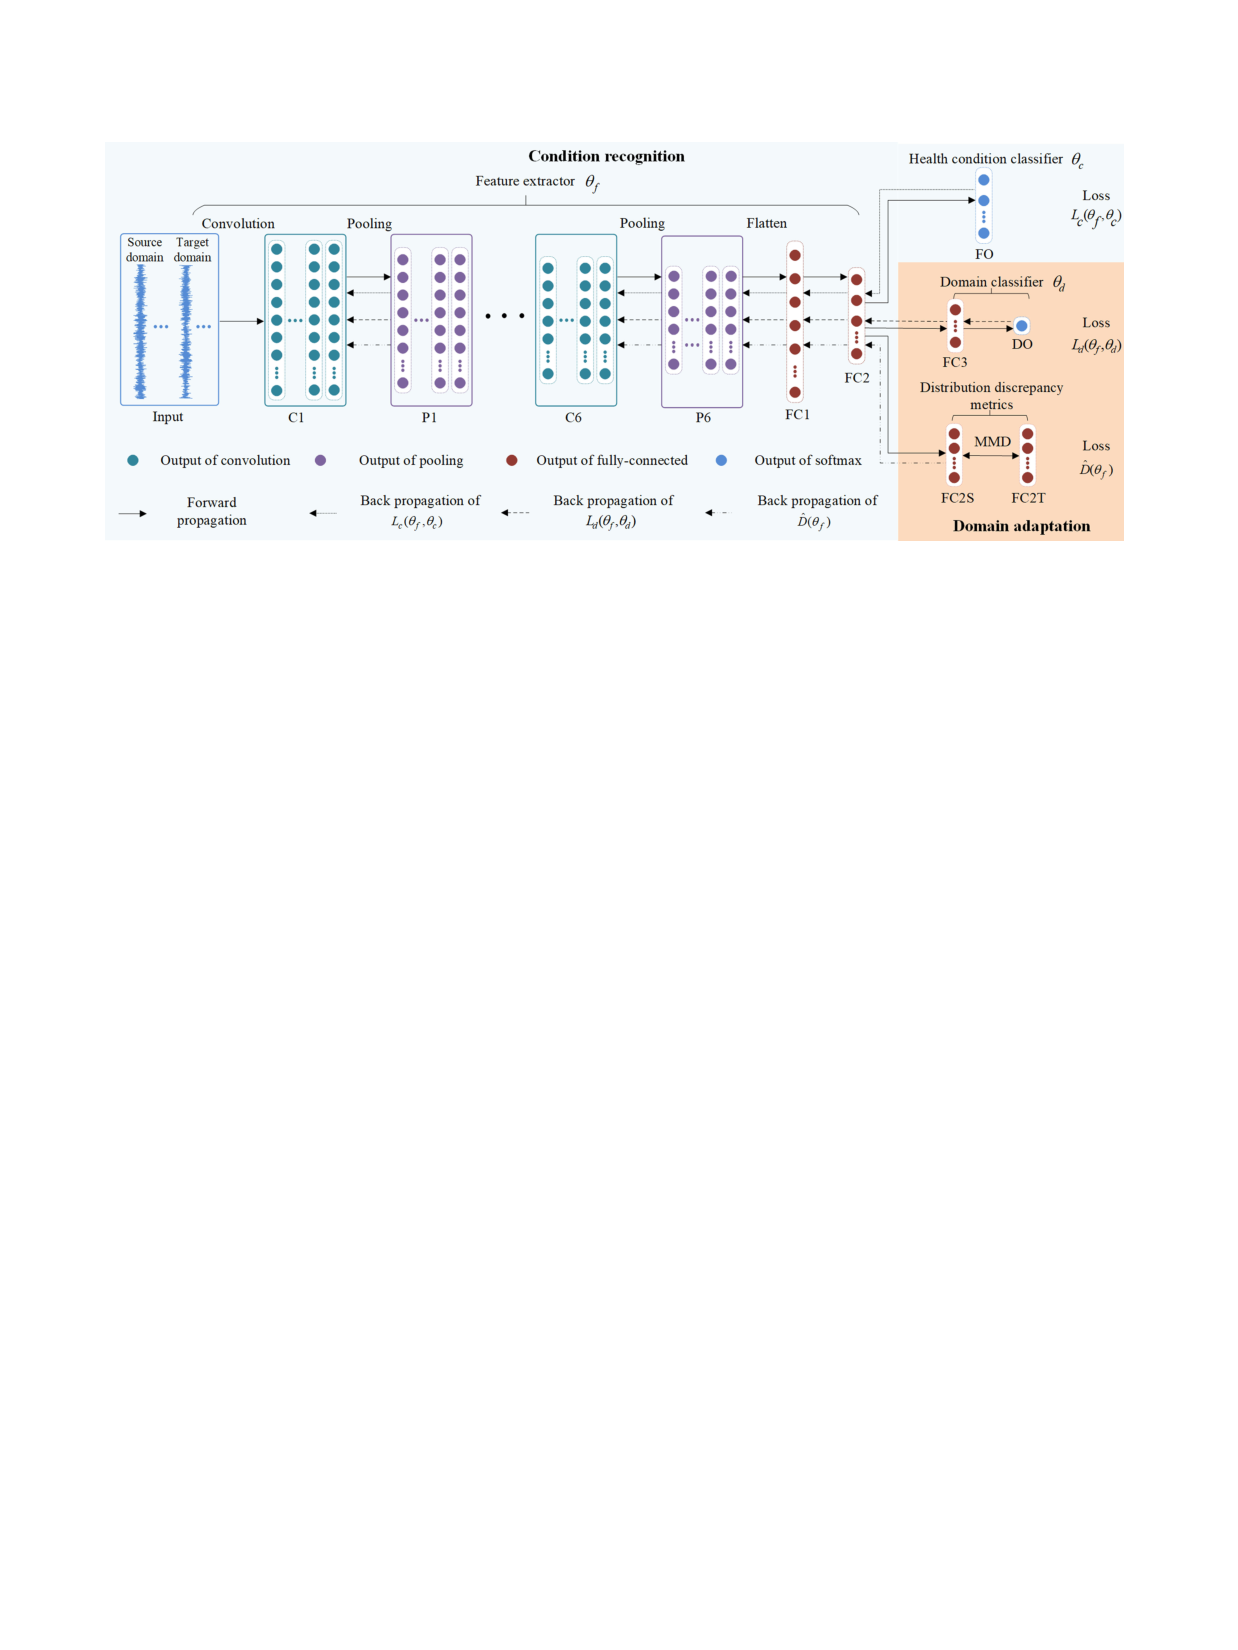
\includegraphics[width=1\textwidth]{models_state_of_the_art/DCTLN_model.pdf}
  \caption{DCTLN model proposed by Guo et al \cite{Guo2019}}
  \label{fig:DCTLN_model}
\end{figure}

\end{comment}

\subsection{Deep Domain Adaption based on MMD-Loss}
Azamfar et al \cite{AZAMFAR2020103932} propose a deep learning based domain adaption approach for BSD PHM, based on a MMD-loss. An experimental test rig was build, containing a single horizontal guideway and a BSD fixed on a concrete base. Three accelerometers were installed to measure vibrations in X and Y directions. These sensors were mounted on the BSD nut and the bottom and top attachments of the BSD shaft. A sound pressure sensor captures the acoustic level when running experiments on the test rig. The torque and speed signals are acquired from the controller. In the experiments the guideways and BSDs are available in three different degradation classes. In the "normal" class the concerned component is operating normally, in the "faulty level 1" class it is deviating from the healthy condition and in the "faulty level 2" class it must be replaced or repaired. In total nine different combinations of guideways and BSDs with different levels of degradation can be combined. Azamfar et al acquire data by performing a full cycle of BSD operation, which contains two full forward and backward movements along the guideways. The data from each recording is split in phases with constant (forward, backward movement) and changing BSD nut velocity (turning point at the end of BSD shaft). The training is restricted to the signals recorded during the phases with constant speed. The data is not split in windows, such that each recorded phase is fed to the model as a single input. The data dimension is reduced by a simple down-sampling method. The full cycle of BSD operation was recorded with different BSD velocities (200, 400 and 600 mm/s). The data distribution discrepancy in the recordings with different BSD velocities creates am domain shift. The proposed method is evaluated on a 9 class classification taks, including all combinations of BSD and guideway degradation classes. The proposed neural network is presented in fig. \ref{fig:Azamfar_model}. It contains a feature extractor of four alternating one-dimensional convolutional and max-pooling layers and a subsequent classifier. The dropout technique with the rate of 0.3 was used to prevent overfitting. The ReLU activation function was used throughout the network. The model is optimized with a source CE-loss to improve the classification accuracy on the source domain data. Besides that the domain discrepancy is reduced by a MMD loss applied in the penultimate fully connected layer. 

\begin{figure}[H]
  \centering
  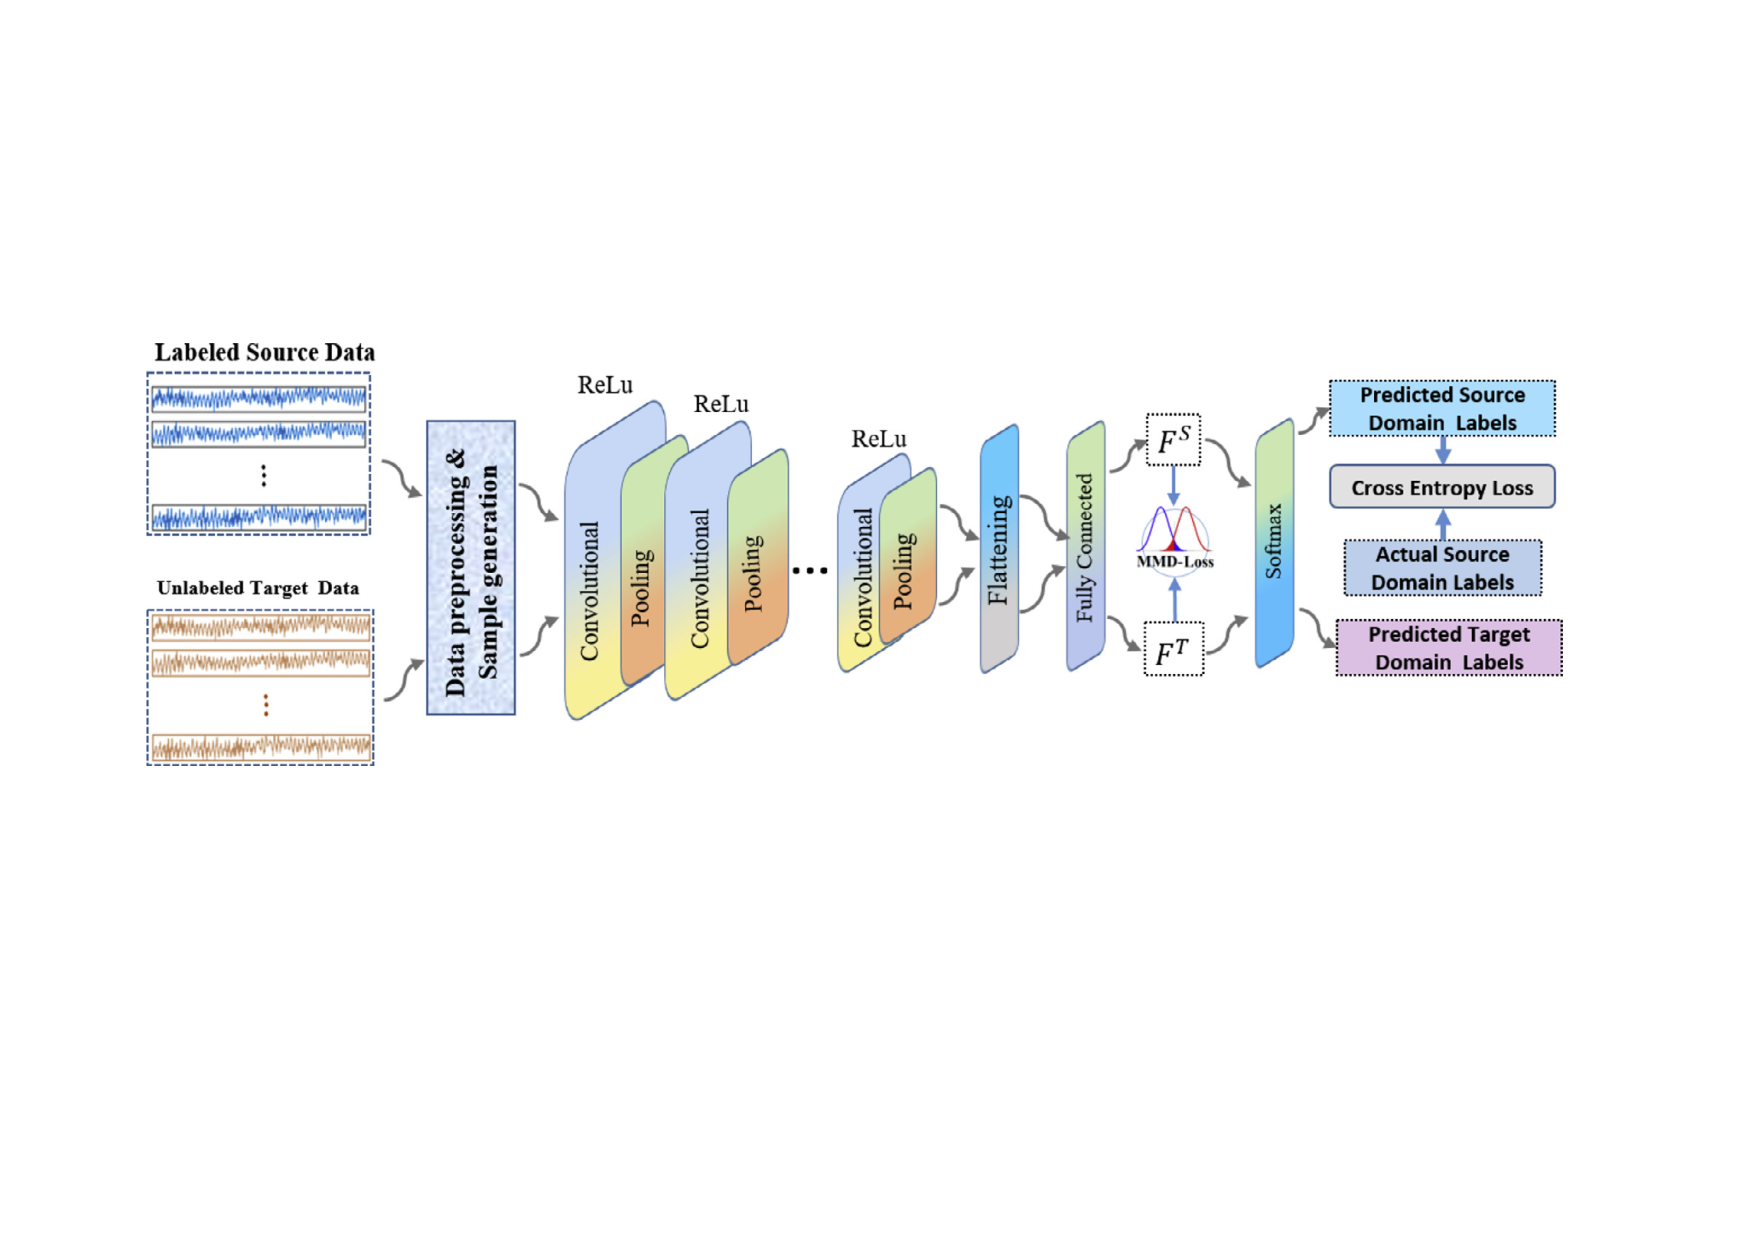
\includegraphics[width=1\textwidth]{models_state_of_the_art/Azamfar_model.pdf}
  \caption{Architecture proposed by Azamfar et al \cite{AZAMFAR2020103932}}
  \label{fig:Azamfar_model}
\end{figure}


\subsection{Deep Domain Adaption based on MMD-Loss and PD Allignment}
Pandhare et al \cite{Pandhare2021} propose a deep learning based domain adaption approach for BSD PHM, based on a MMD-loss and PD allignment. An identical test rig, as the one presented by Azamfar et al \cite{AZAMFAR2020103932}, was used by Pandhare et al to evaluate the proposed models. In total, five accelerometers were mounted in the test bed. Two triaxial ones were placed close to the BSD nut, which seems a promising position to represent the signature of a ball screw preload level. Three single-axial ones were mounted at the bottom and top attachments of the BSD shaft and on top of the load carried by the BSD nut. The last three sensor positions are chosen due to their more suitable and practical installation. Identical to Azamfar et al \cite{AZAMFAR2020103932} nine combinations of degradation classes of BSD and guideways are defined. The proposed model should overcome the domain discrepancy between datasets generated with differently mounted sensors. The goal of the work is to find an indirect sensing method to make PHM on BSDs independent of impractical sensor locations. The proposed model is presented in fig. \ref{fig:Pandhare_model} and contains a feature extractor of two convolutional and max pooling layers and a consecutive classifier. The proposed model training includes three losses. Again, a source CE-loss is used to improve the classification performance on the source domain data. The MMD loss reduces the marginal distribution mismatch between the domains. The PD alignment reduces the conditional distribution discrepancy of the domains. This is done by matching source and target samples with equal class label and reducing their L2-distance: 

\begin{equation}
    L_{p} = \frac{1}{n_{p}}\sum_{k=1}^{n_{p}}|h_{k}^{p,s}-h_{k}^{p,t}|_{2}, 
\end{equation}
where $h_{k}^{p,s}$ and $h_{k}^{p,t}$ are the k-th source and target domain samples and $n_{p}$ is subspace of the labeled samples from source and target. 

\begin{figure}[H]
  \centering
  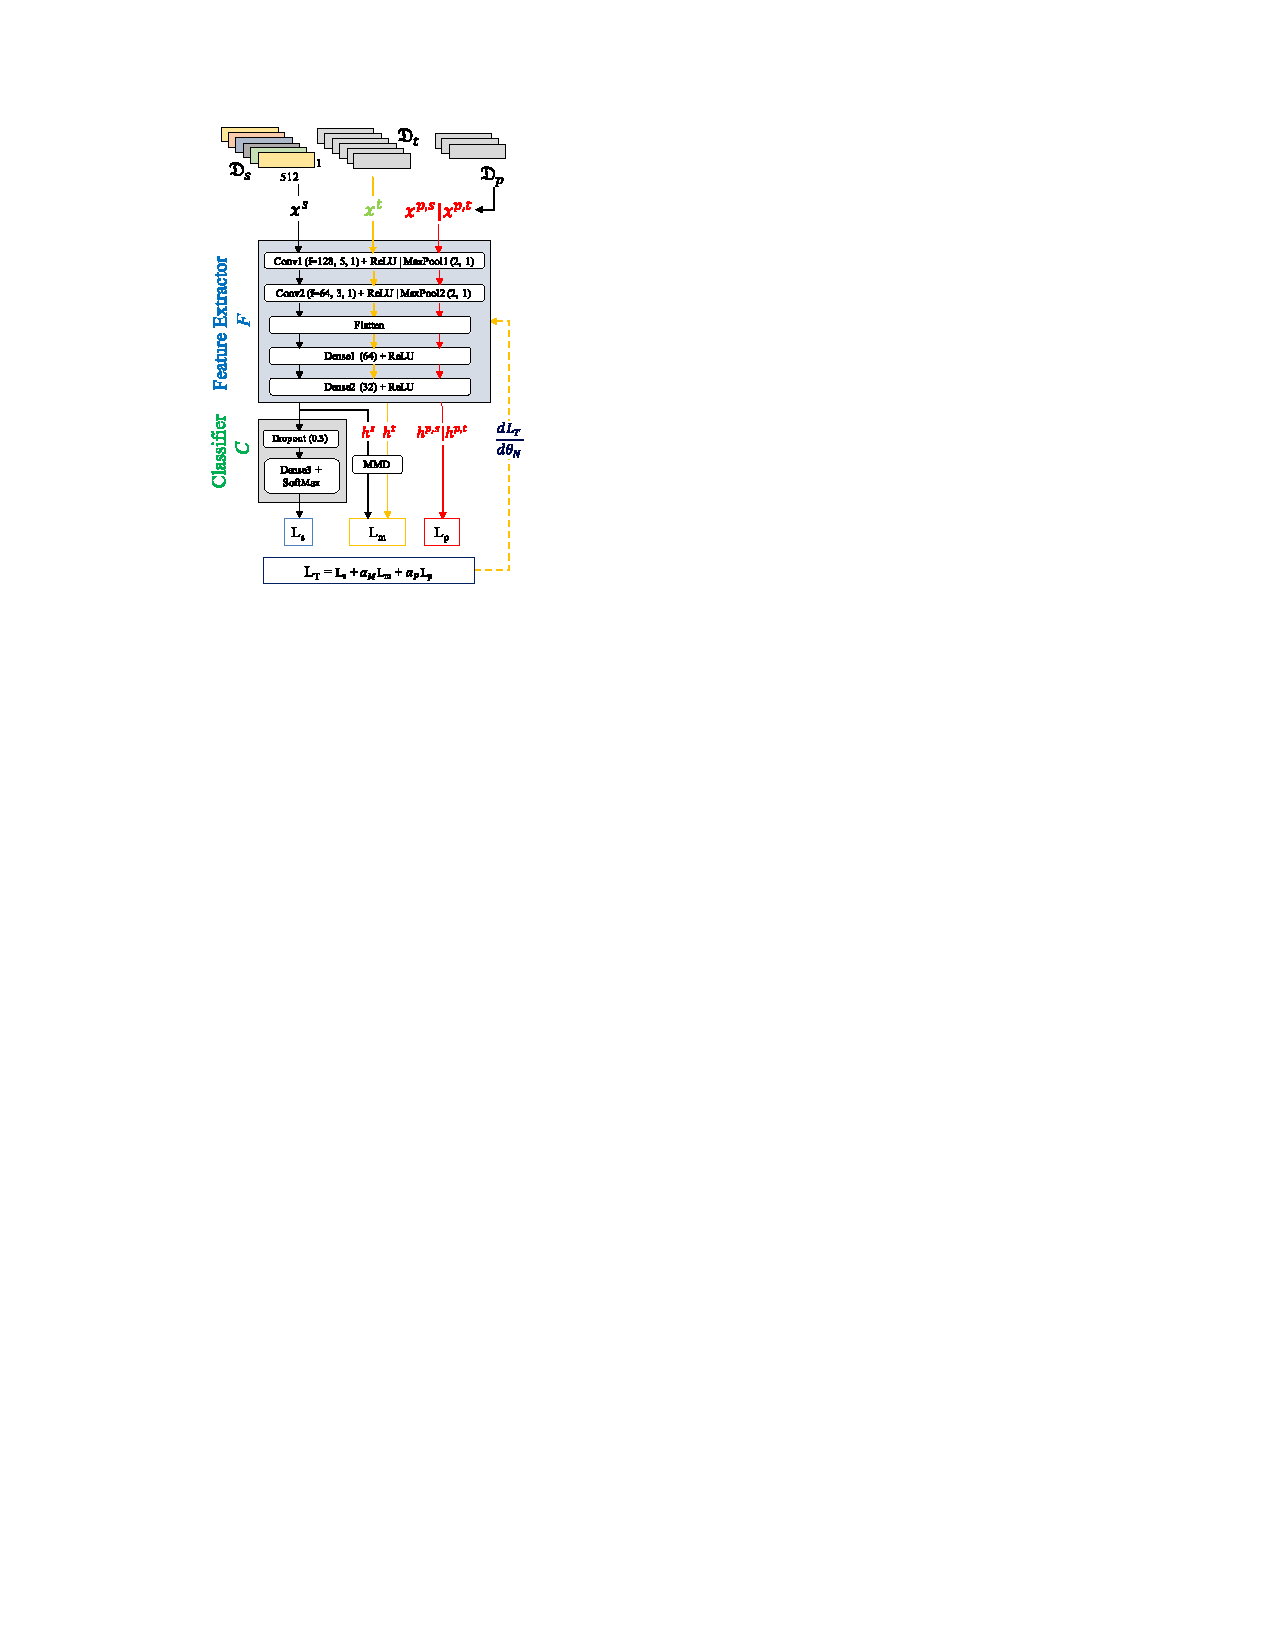
\includegraphics[width=.6\textwidth]{models_state_of_the_art/Pandhare_model.pdf}
  \caption{Architecture proposed by Pandhare et al \cite{Pandhare2021}}
  \label{fig:Pandhare_model}
\end{figure}
\begin{comment}
\subsection{Domain Conditioned Adaptation Network}
Most domain adaption approaches reduce the domain discrepancy in task-specific layers but use a shared feature extractor backbone across all domains. Li et al \cite{li2020} assume that, if the domain discrepancy is tremendously large, these methods can only reduce the domain discrepancy, but not fundamentally eliminate it. In the proposed Domain Conditioned Adaptation Network (DCAN) Li et al present some alternative and more effectively domain adaptive approach. Li et al recommend to extract domain-specific and -independent features in the feature extractor backbone. Since the source and target domains are correlated to some extend, the network itself can extract domain-independent features. The powerful feature extractor learned from the source domain can also increase the model performance on the target domain. At the same time, features which are too sensitive to the source domain can even reduce the model performance on the target domain. To counteract that phenomena, Li et al recommend to additionally extract domain-specific features in the convolutional layers. This can improve the cross-domain feature alignment in the task-specific layers. A domain conditioned feature correction module is applied to reduce the domain discrepancy in the extracted domain-specific and -independent features. Additionally, the model is optimized with a conventional supervised source and a newly proposed unsupervised target CE-loss defined as following:

\begin{equation}
    \min_{G} L_{s} = -\frac{1}{n_{t}} \sum_{j=1}^{n_{t}} \sum_{k=1}^{C_{n}} G^{(k)}(\pmb{x}_{tj})logG^{(k)}(\pmb{x}_{tj}),
\end{equation}
where $G(\cdot)$ is the learned predictive model, $n_{t}$ the number of source domain samples, $C_{n}$ the classes present in source and target domain and $\pmb{x}_{t}$ the target samples. The presented model is developed for computer vision applications and is never been evaluated in the context of PHM. Since PHM suffers from similar problems, this approach might be relevant and interesting for the PHM community. The model is visualized in fig. \ref{fig:DCAN_model}. In the following, the two domain adaption modules are described in more detail \cite{li2020}. 

\subsubsection{Domain Conditioned Channel Attention Mechanism}
Li et al \cite{li2020} use ResNet as backbone network, which allows an easy implementation of the domain conditioned channel attention module in its residual block. In the latent feature maps the processed images are represented as $\pmb{X}_{t} = [X^{1}_{t},...,X^{C}_{t}] \in \mathbb{R}^{HxWxC}$, where H and W are the spatial dimension and C the number of image channels. First, a channel-wise global average pooling layer is applied which reduces the images to  $\pmb{g}_{t} = [g^{1}_{t},...,g^{C}_{t}] \in \mathbb{R}^{1x1xC}$. Afterwards, the data is split depending on its domain and passed through different fully connected layers. The upper flow is used for target and the lower flow for source domain samples. The two different source and target domain routes share parameters. For both domains, an attention mechanism is trained jointly to learn activating different channels in the domain samples. This allows extracting more enriched domain specific features. In the fully connected layers the dimension is first reduced with a ratio ${1x1x\frac{C}{r}}$ and later reconstructed to its original size ${1x1xC}$. Relu and Sigmoid functions are applied. The domain-wise feature selection is achieved by weighting the channels of the feature representations $\pmb{X}_{s}$ and $\pmb{X}_{t}$ with the channel attention vectors $\pmb{v}_{s}$ and $\pmb{v}_{t}$ calculated by the domain conditioned channel attention module:

\begin{equation}
    \begin{aligned}
        &\pmb{\tilde{X}}_{s} = \pmb{v}_{s} \odot \pmb{X}_{s} = [v_{s}^{1} \cdot X_{s}^{1}, ..., v_{s}^{C} \cdot X_{s}^{C}]\\
        &\pmb{\tilde{X}}_{t} = \pmb{v}_{t} \odot \pmb{X}_{t} = [v_{t}^{1} \cdot X_{t}^{1}, ..., v_{t}^{C} \cdot X_{t}^{C}].
    \end{aligned}
\end{equation}

The domain conditioned channel attention module allows the model to independently learn the importance of each channel for the classification of source and target domain samples \cite{li2020}.


\subsubsection{Domain Conditioned Feature Correction}
A feature correction block is placed after each of the l task-specific layers to counteract the decreasing transferability in high-level features. At the feature correction blocks, the data simultaneously passes through the regular network and the feature correction block, which consist of FC and Relu blocks. The feature correction block estimates the domain discrepancy in the feature representation of the task-specific layer:
\begin{equation}
    \Delta H_{l}(x_{t}) = H_{l}(x_{s}) - H_{l}(x_{t}),
\end{equation}
where $H_{l}(x_{s})$ and $H_{l}(x_{t})$ are the feature representations of the source and target domain samples in the task-specific layer l and $\pmb{x}_{s}$ and $\pmb{x}_{t}$ the source and target domain samples. The feature representation of the target domain samples is corrected as following:
\begin{equation}
    \hat{H}_{l}(x_{t}) = H_{l}(x_{t}) + \Delta H_{l}(x_{t}).
\end{equation}


The discrepancy between the regular feature representation of source domain samples $H_{l}(x_{s})$ and the corrected feature representation of the target domain samples $\hat{H}_{l}(x_{t})$ is measured with a MMD-loss in several layers:

\begin{equation}
    L_{M}^{l} = |\frac{1}{n_s} \sum_{i=1}^{n_{s}} \phi(H_{l}(x_{si}) - \frac{1}{n_t} \sum_{i=1}^{n_{t}} \phi(\hat{H}_{l}(x_{ti}))|_{H_{\kappa}}^{2}, 
\end{equation}
where $H_{\kappa}$ is the reproducing kernel Hilbert space (RKHS), $\kappa$ the characteristic kernel and $\phi$ corresponding feature map. The number of source and target samples is defined by $n_{s}$ and $n_{t}$. Reducing the domain discrepancy improves the feature transferability, but also transfers noise and unimportant information between the domains. This destroys the structure of the source and target domain data and makes the classification task even more difficult. To avoid this over-transfer between source and target, the model is enforced to keep the source data constant when passing through the feature correction blocks. Since $\Delta H_{l}(x_{s}) \approx 0$ would prevent the cross-domain feature correction, another regularization term tackles that problem:
\begin{equation}
    L_{reg}^{l} = \sum_{k=1}^{C_{n}}|\frac{1}{n_{s}^{k}} \sum_{x_{si} \in S^{k}} \phi(H_{l}(x_{si})) - \frac{1}{|R|} \sum_{x_{sj} \in R} \phi(\hat{H}_{l}(x_{sj}))|_{Hk}^{2}, 
\end{equation}
where $R$ is a random subset of source domain samples and $S^{k}$ is the set of source domain samples belonging to class k \cite{li2020}.

\begin{figure}[H]
  \centering
  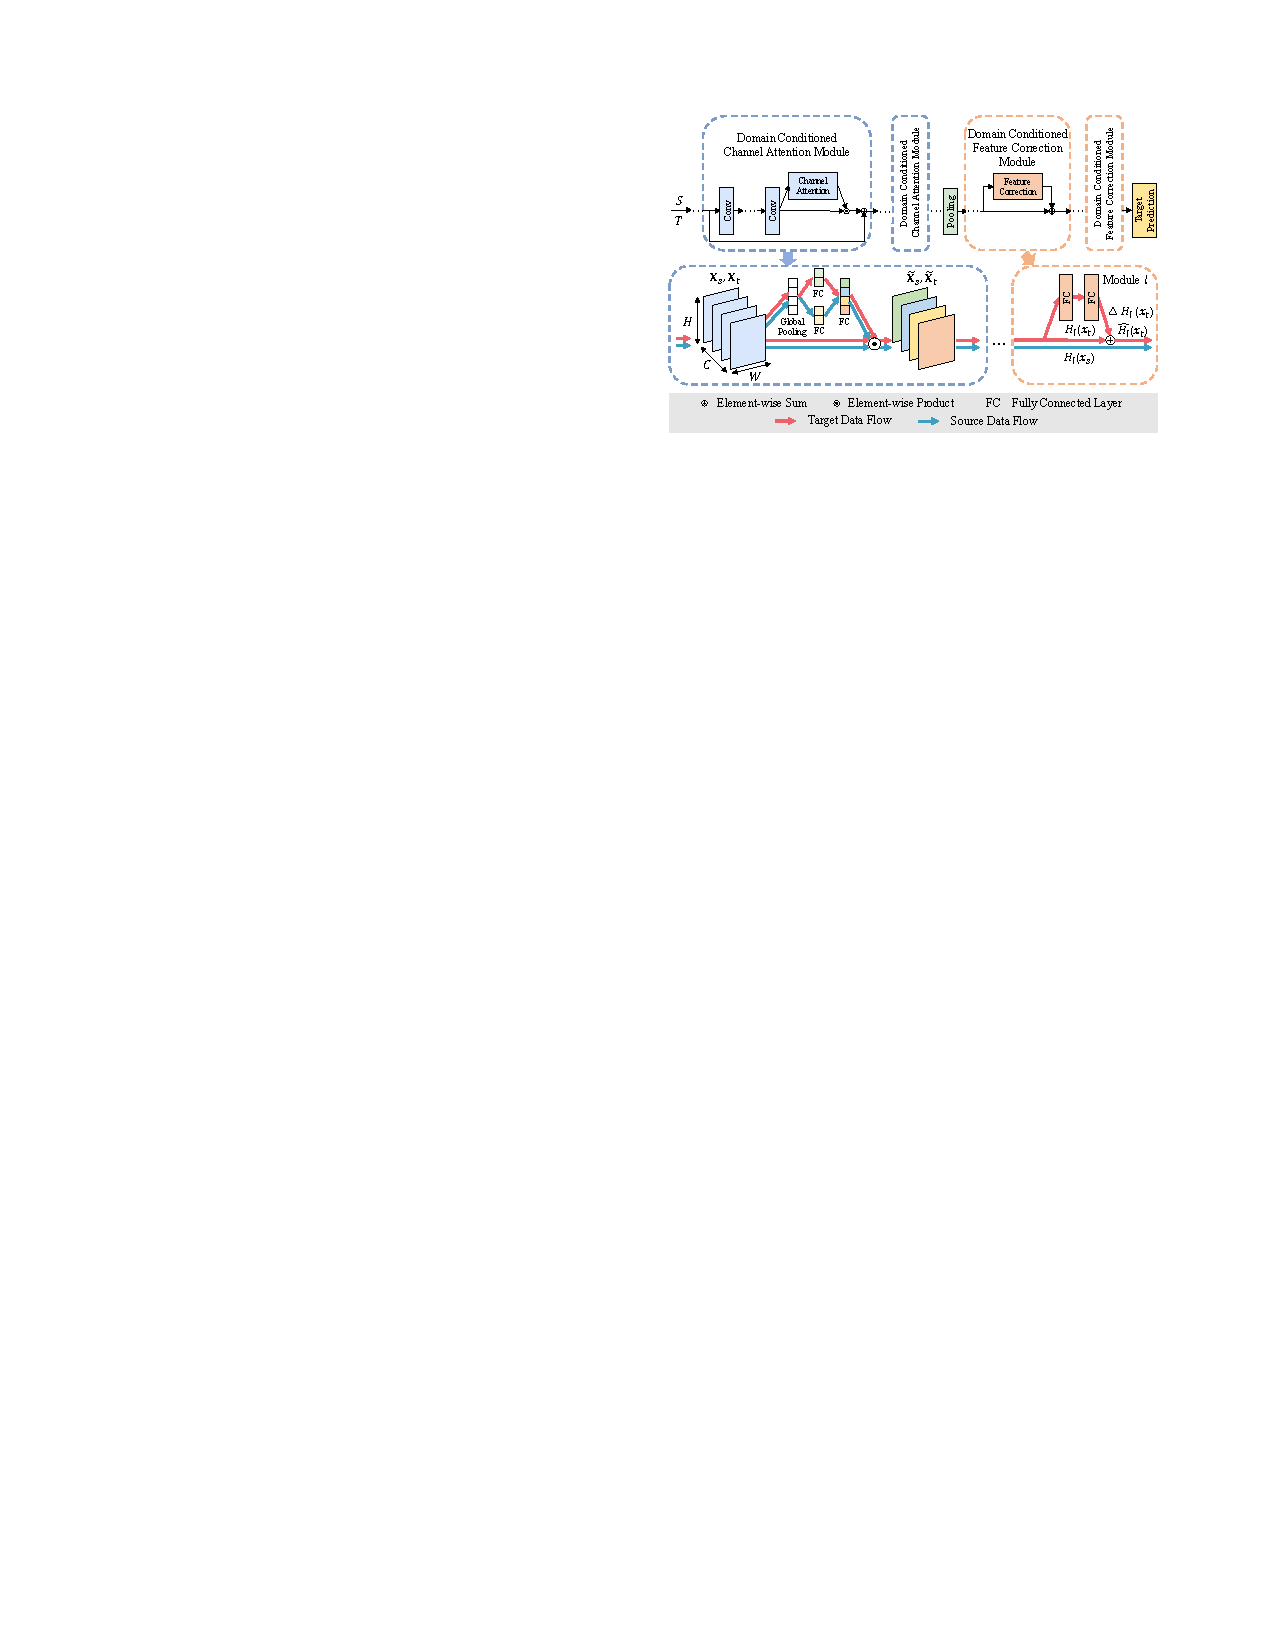
\includegraphics[width=1\textwidth]{models_state_of_the_art/DCAN_model.pdf}
  \caption{DCAN architecture proposed by Li et al \cite{li2020}}
  \label{fig:DCAN_model}
\end{figure}
\end{comment}



\begin{comment}

\subsection{Wasserstein Distance Guided Multi-Adversarial Network}
Zhang et al \cite{Zhang2019} present a Wasserstein distance guided multi-adversarial network (WDMAN) for rolling bearing fault diagnosis under different working conditions. The proposed architecture consists of a CNN feature mapper and a subsequent classifier. In the fully connected layers of the classifier, several Domain Critic Networks estimate the domain discrepancy by applying the Wasserstein-distance. A source CE-loss is applied in the end of the network. The whole model and the applied losses are visualized in fig. \ref{fig:WDMAN_model}.

 \begin{figure}[H]
  \centering
  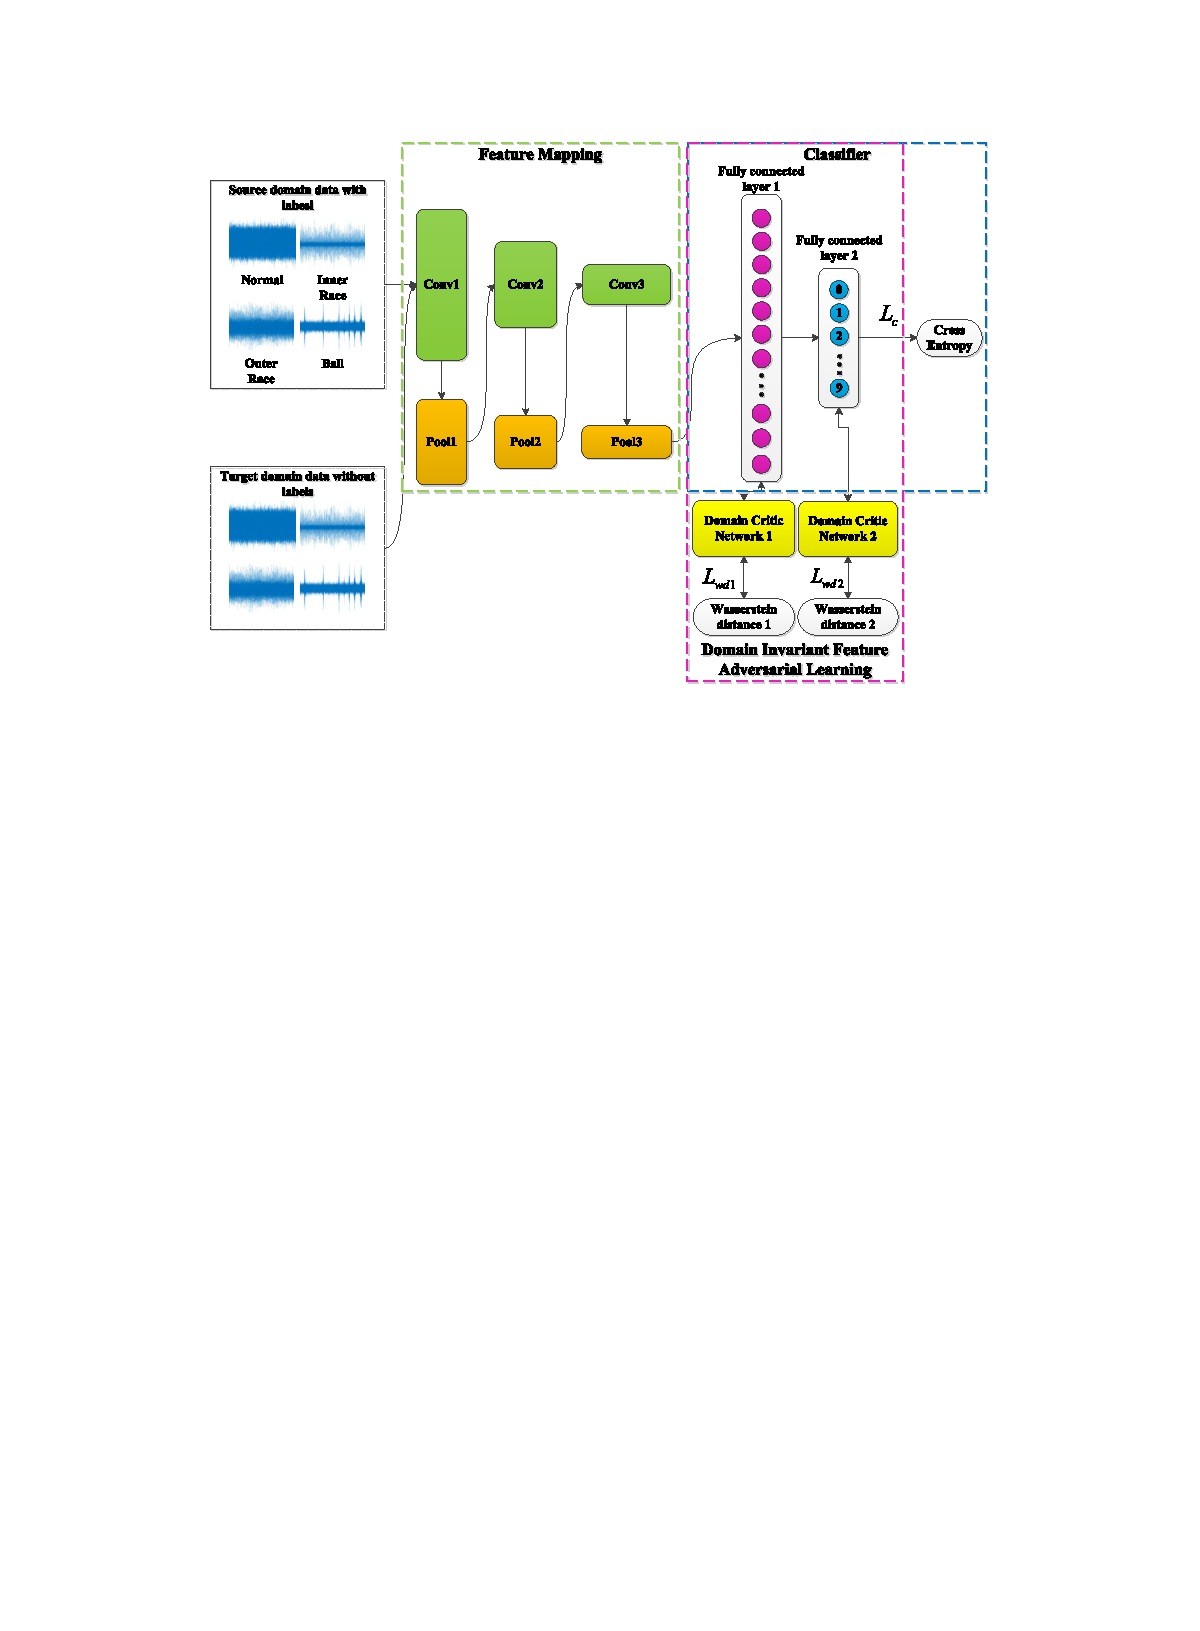
\includegraphics[width=1\textwidth]{models_state_of_the_art/WDMAN_model.pdf}
  \caption{WDMAN architecture proposed by Zhang et al \cite{Zhang2019}}
  \label{fig:WDMAN_model}
\end{figure}

In a pre-training phase, the feature mapper $\theta_{M}$ and classifier $\theta_{C}$ are optimized with the source CE-loss:
 
\begin{equation}
     L_{c}(x^{s}, x^{t}) = -\frac{1}{n^{s}} \sum_{i=1}^{n^{s}} \sum_{k=1}^{K} l(y_{i}^{s}=k) \cdot logC(M(x_{i}^{s}))_{k},
\end{equation}

where $n^{s}$ is the number of source samples, $K$ is the number of classes, $x_{i}^{s}$ and $y_{i}^{s}$ are the source samples and corresponding labels, $M(\cdot)$ and $C(\cdot)$ are the feature mapper and classifier. In the adversarial training afterwards, the model learns to extract more domain invariant features by minimizing the Wasserstein distance in the fully connected layers of the classifier. The domain critic networks try to maximize and the feature mapper to minimize the adversarial loss. The adversarial training transfers the model, trained on the source domain, to the target domain:
 
\begin{equation}
     L_{wd}(x^{s}, x^{t}) = \frac{1}{n^{s}} \sum_{x^{s} \in X^{s}} D(F(x^{s})) - \frac{1}{n^{t}} \sum_{x^{t} \in X^{t}} D(F(x^{t})),
\end{equation}

where $x^{s}$ and $x^{t}$ are the data samples drawn from the source domain $X^{s}$ and target domain $X^{t}$. The feature representations of the source and target samples in the fully connected layers are denoted as $F(\cdot)$. The domain critic networks are represented by $D(\cdot)$. In the adversarial learning, the model and discriminators are optimized in an alternating procedure:

\begin{equation}
    \min_{\theta_{F}} \max_{\theta_{D}} (L_{wd} - \lambda L_{gp}), 
\end{equation}

where $\theta_{F}$ and $\theta_{D}$ are the parameters of the feature mapper and domain critics, $\lambda$ is the penalty coefficient. Generally, the goal of the discriminators is to identify the domain of each sample. The feature mapper tries to extract domain-independent features, which precludes the discriminator predicting the correct domain. To satisfy the Lipschitz constraint condition of the Wasserstein distance, an additional gradient penalty is applied: 

\begin{equation}
     L_{gp}(\tilde{x}) = (|\nabla_{\tilde{x} \in P_{\tilde{x}}} D(\tilde{x})|_{2}-1)^{2}, 
\end{equation}
where $P_{\tilde{x}}$ is a distribution of samples coming from the line connecting a pair of points sampled from the source and target domain. The Wasserstein distance is extended with the gradient penalty. The workflow of the model is described more detailed in fig. \ref{fig:WDMAN_workflow}
 
\begin{figure}[H]
  \centering
  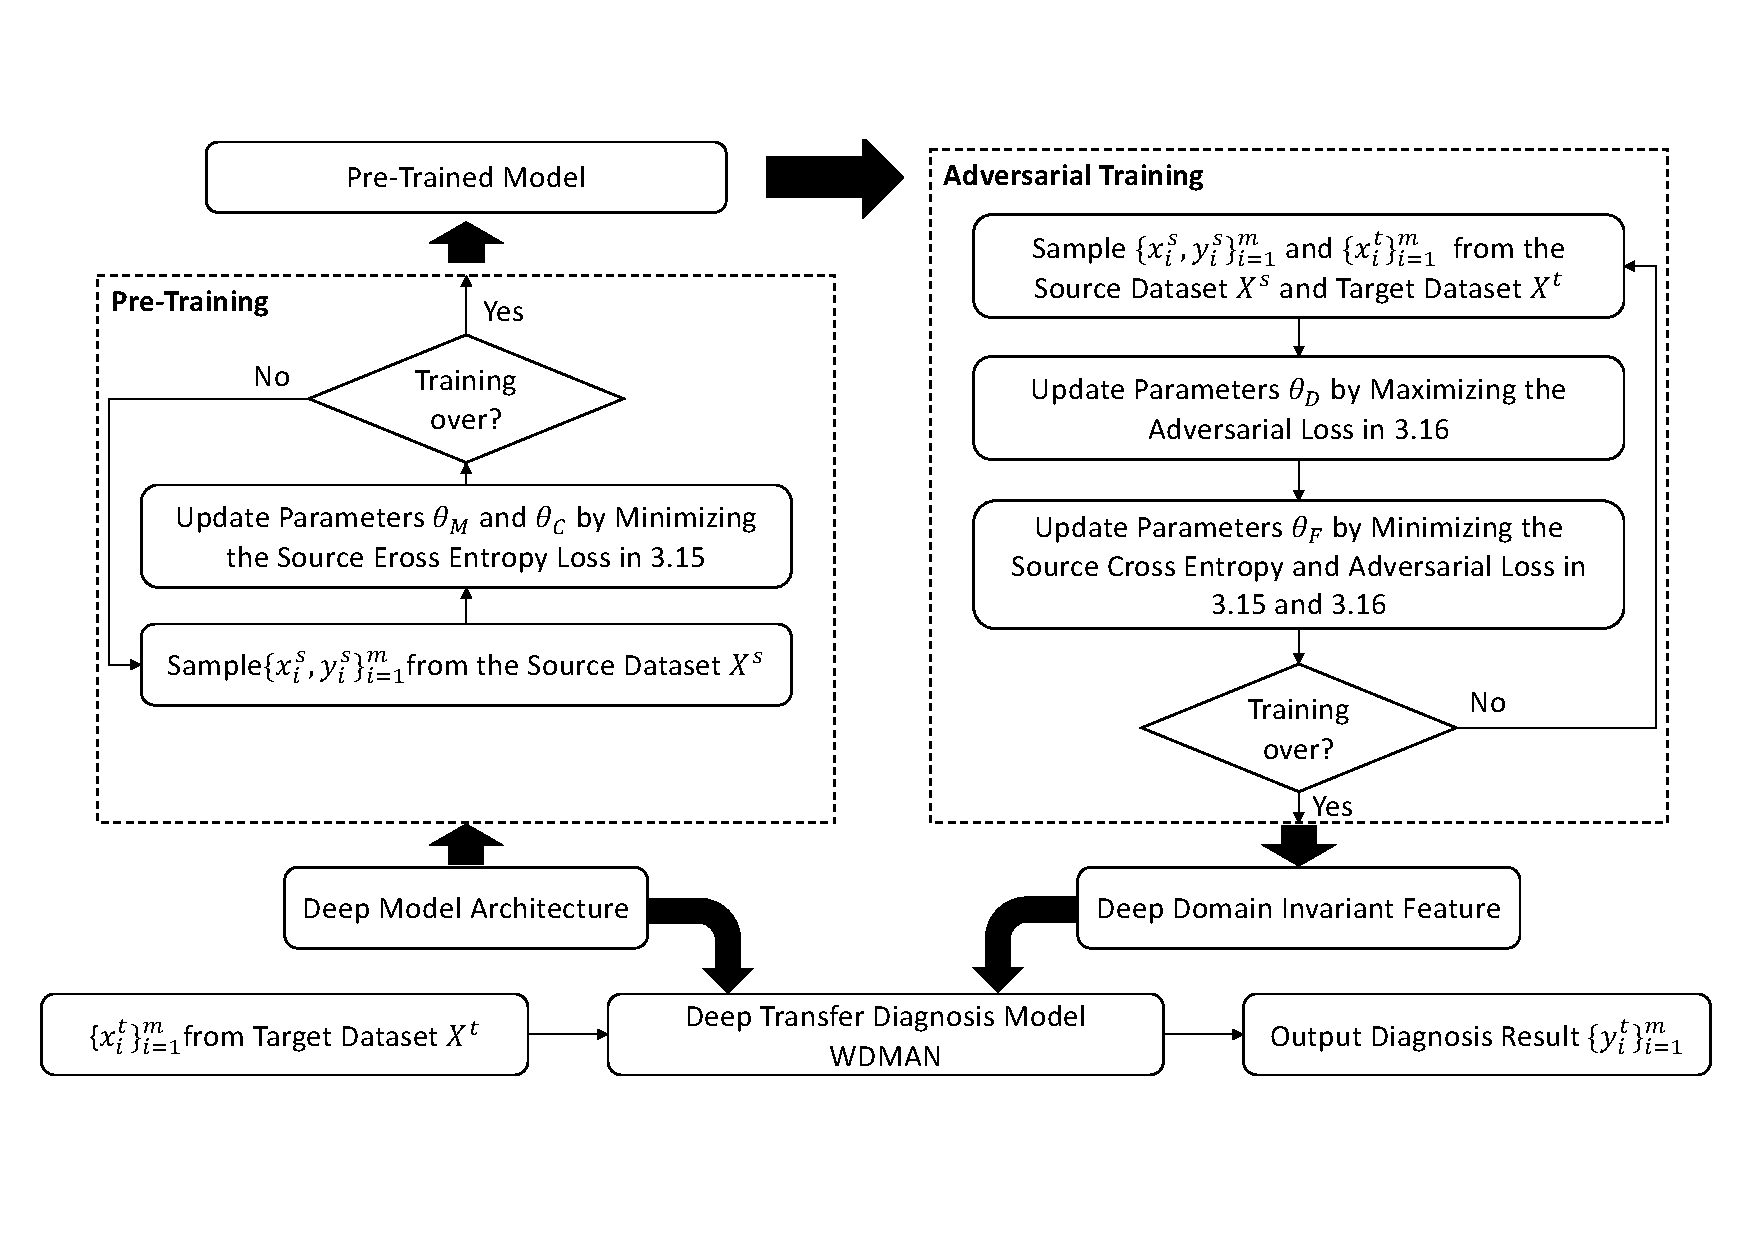
\includegraphics[width=.9\textwidth]{models_state_of_the_art/WDMAN_workflow.pdf}
  \caption{WDMAN workflow based on \cite{Zhang2019}}
  \label{fig:WDMAN_workflow}
\end{figure}
 
 
\end{comment}